\section{Theoretical Models}
\subsection{Capital Asset Pricing Model (CAPM)}
The Capital Asset Pricing Model (CAPM) is employed to determine the expected return on an asset based on its systematic risk, as measured by beta ($\beta_i$). The CAPM formula is:

\[
E(R_i) = R_f + \beta_i (E(R_m) - R_f)
\]

where \( R_f \) is the risk-free rate, \( E(R_m) \) is the expected return of the market portfolio, and \( \beta_i \) is the asset’s beta, reflecting its sensitivity to market movements. This model facilitates the estimation of expected returns required for the portfolio optimization process.

\subsubsection{Beta Calculation}
Beta ($\beta_i$) measures the volatility of an asset in relation to the market. It is calculated as:

\[
\beta_i = \frac{\text{Cov}(R_i, R_m)}{\sigma^2_m}
\]

where \(\text{Cov}(R_i, R_m)\) is the covariance between the asset return \( R_i \) and the market return \( R_m \), and \( \sigma^2_m \) is the variance of the market return.

\subsubsection{Security Market Line (SML)}
The Security Market Line (SML) is a graphical representation of the Capital Asset Pricing Model (CAPM), showcasing the relationship between the expected return of an asset and its systematic risk, as measured by beta ($\beta_i$). The SML illustrates the expected return of a security at different levels of systematic risk. The equation of the SML is given by CAPM:

\[
E(R_i) = R_f + \beta_i (E(R_m) - R_f)
\]

where:
\begin{itemize}
    \item \( E(R_i) \) is the expected return of the asset,
    \item \( R_f \) is the risk-free rate,
    \item \( \beta_i \) is the beta of the asset,
    \item \( E(R_m) \) is the expected return of the market portfolio.
\end{itemize}

The SML provides a benchmark for evaluating the performance of individual securities. Securities plotted above the SML are considered undervalued as they offer higher returns for a given level of risk. Conversely, securities below the SML are considered overvalued as they offer lower returns for the same level of risk.

\subsubsection{Theoretical Implications}
The SML conveys several important theoretical implications:
\begin{itemize}
    \item All securities, when correctly priced, should lie on the SML.
    \item The slope of the SML is the market risk premium, \( E(R_m) - R_f \), representing the additional return expected from holding a market portfolio instead of risk-free assets.
    \item The intercept of the SML is the risk-free rate, \( R_f \), reflecting the return of a theoretically risk-free asset.
\end{itemize}

\begin{figure}[h]
\centering
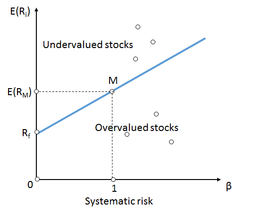
\includegraphics[width=0.5\textwidth]{SML.png} 
\caption{Security Market Line. Source: \href{https://en.wikipedia.org/wiki/Security_market_line}{Wikipedia}}
\label{fig:sml}
\end{figure}

The SML is a fundamental concept in our next topic of modern portfolio theory, aiding investors in making informed decisions about asset allocation based on expected returns and systematic risks.

\subsection{Modern Portfolio Theory}
Modern Portfolio Theory provides a robust framework for constructing an optimal portfolio that maximizes expected return for a given level of risk. The expected return \( E(R_p) \) of a portfolio is the weighted sum of the expected returns of the individual assets:

\[
E(R_p) = \sum_{i=1}^{n} w_i E(R_i)
\]

where \( w_i \) is the weight of asset \( i \) in the portfolio, and \( E(R_i) \) is the expected return of asset \( i \). The portfolio’s variance \( \sigma^2_p \), representing its risk, is given by:

\[
\sigma^2_p = \sum_{i=1}^{n} \sum_{j=1}^{n} w_i w_j \sigma_{ij}
\]

where \( \sigma_{ij} \) is the covariance between the returns of assets \( i \) and \( j \). This formulation allows for the identification of efficient portfolios that lie on the efficient frontier, representing the optimal trade-offs between risk and return.

\subsubsection{Efficient Frontier and Optimal Portfolio}
The efficient frontier is a concept from MPT that represents the set of optimal portfolios offering the highest expected return for a defined level of risk. The process of constructing the efficient frontier involves solving the following optimization problem:

\[
\min \sum_{i=1}^{n} \sum_{j=1}^{n} w_i w_j \sigma_{ij}
\]

subject to:
\[
\sum_{i=1}^{n} w_i = 1
\]

and
\[
E(R_p) = \sum_{i=1}^{n} w_i E(R_i)
\]

\begin{figure}[h]
\centering
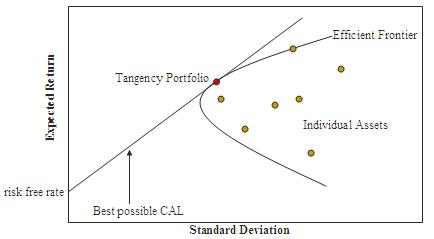
\includegraphics[width=0.5\textwidth]{efficient_frontier.png} 
\caption{Efficient Frontier of Optimal Portfolios. Source: \href{https://en.wikipedia.org/wiki/Efficient_frontier}{Wikipedia}}
\label{fig:efficient_frontier}
\end{figure}


\subsection{Monte Carlo Simulation}
Monte Carlo simulations are utilized to model the uncertainty and variability in investment returns over time. The simulation process involves generating random returns based on historical data and iterating this process to build a distribution of potential outcomes. The value of an investment at time \( i \) is given by:

\[
X_i = X_{i-1} \times (1 + r_i)
\]

where \( X_i \) is the investment value at time \( i \) and \( r_i \) is the return for period \( i \). By running multiple simulations, we can estimate the expected value and variability of the investment portfolio, providing insights into the likelihood of achieving the desired down payment amount within the specified time horizon.

\subsubsection{Simulation Algorithm}
The Monte Carlo simulation algorithm follows these steps:
\begin{enumerate}
    \item Initialize the investment value \( X_0 \).
    \item For each time step \( i \), generate a random return \( r_i \) from the historical return distribution.
    \item Update the investment value: \( X_i = X_{i-1} \times (1 + r_i) \).
    \item Repeat steps 2 and 3 for the desired number of time steps.
    \item Aggregate the results to build a distribution of potential outcomes.
\end{enumerate}

\subsubsection{Expected Value and Variance Calculation}
The expected value \( E(X) \) and variance \( \sigma^2(X) \) of the investment outcomes are calculated as:

\[
E(X) = \frac{1}{N} \sum_{i=1}^{N} X_i
\]

\[
\sigma^2(X) = \frac{1}{N - 1} \sum_{i=1}^{N} (X_i - E(X))^2
\]

These calculations provide a quantitative measure of the potential outcomes of the investment strategies, allowing for the assessment of risk and return profiles.

\subsection{Implications for the Business Problem}
The theoretical models described above provide a structured approach to constructing and evaluating investment portfolios aimed at accumulating housing down payments. The Modern Portfolio Theory ensures that the portfolios are optimized for maximum returns at a given risk level, while the CAPM helps in understanding the risk-return trade-off specific to each asset. The Monte Carlo simulations add a layer of probabilistic analysis, offering insights into the range of possible outcomes and their associated probabilities.

The implications for the business problem are significant. By employing these models, first-time homebuyers can design their own personalized investment strategies that cater to their unique risk tolerance and time horizons. This can lead to more effective savings plans, ultimately making homeownership more attainable.

